\chapter{更新Ren'Py}

\begin{ChapterGoals}
    \begin{itemize}
        \item 更新你的Ren'Py版本;
        \item 学会解除兼容性警告。
    \end{itemize}
\end{ChapterGoals}

首先,恭喜您完成了基础篇的学习,来到了进阶篇。在进入正文以前,我们不得不提醒您需要有一定的Python基础才能完成进阶篇的学习。仅靠本书浅显的介绍是远远不够的,因此,我们建议您在进行一段时间的模组开发和Python学习后再来阅读本部分。

本章我们将会学习如何将您的模板更新的Future分支以启用更多功能,并使用Ren'Py 8进行进一步的开发。

\begin{Warning}
    请注意,目前DDLC中文模板已经有2年未更新,最新版本的Ren'Py不一定能够完美适配模板。若Ren'Py 8后续版本进行了不兼容的修改,可能会让模板运行错误。因此我们推荐您使用最后一个确定适配的版本——Ren'Py 8.0.3。但最新的Ren'Py 8也带来了一些新特性,为了使用最新版本的Ren'Py 8,我们需要解除兼容性警告。总而言之,本书会向您介绍如何使用最新版本的Ren'Py 8,但本书中的代码只保证能在Ren'Py 8.0.3上正常运行,不保证最新版Ren'Py 8能够成功运行。
\end{Warning}

\section{判断您是否需要升级}
首先,升级模板是一个很复杂的过程。尤其是将模板从Next分支(Python 2版本)升级到Future分支(Python 3)版本。一般来说,您的代码仅需较少的改动或完全不需改动便可迁移到Future分支。但由于Python 2与Python 3、Ren'Py 7与Ren'Py 8之间的差异较大,相同的代码在不同分支上运行可能会有不同的效果。为了判断您是否需要升级,本部分将会给您参考建议,帮助您判断是否需要升级。
请按照以下步骤进行判断:
\begin{enumerate}
    \item 您是否需要或想要使用Ren'Py 8 或 Python 3 的一些新特性(如多线程操作、\ruby{格式化字符串}{f-string}、\ruby{关键词参数}{Keyword-Only Arguments}等)
    \item 您是否有足够的技术修正代码预期外的运行效果
    \item 您能否接受升级到Future分支所\textbf{可能}带来的游戏的不稳定
\end{enumerate}
若以上三个条件均满足,我们建议您升级到Future分支。您也可以出于尝试目的升级您的项目,只要先进行备份。

\section{更新Ren'Py版本与模板版本}
在一切开始之前,请先对您现在的项目文件夹进行备份,只需将您的项目文件夹压缩成压缩包或复制一份即可。

\begin{Warning}
    截止到本章编写时,Ren'Py 7的支持即将结束,故我们建议您直接升级至Future分支与Ren'Py 8版本,而不是停留在Ren'Py 7。
\end{Warning}

\subsection{更新Ren'Py}
更新 Ren'Py 版本是一个相对简单的步骤。首先,前往\url{https://www.renpy.org/latest.html}下载 Ren'Py 8 的最新版本。

然后,按照第\ref{1.2}节完成对Ren'Py的配置。

\subsection{更新模板}
现在,前往\url{https://github.com/DokiMod/DDLCModTemplate-Chinese-future},按照第\ref{2.1.1}节的步骤,下载Future分支并完成配置。

接下来,我们将进入最复杂的一个环节——迁移修改过的代码。
首先,打开VS Code,按照第\ref{2.1.2}节步骤安装Compare Folders插件。随后,使用VS Code打开您项目文件夹所处的文件。例如:我的项目名字叫作“ClubStory”,储存在名为“项目”的文件夹,那么我应该使用VS Code打开“项目”文件夹而非“ClubStory”文件夹。

然后,按照第\ref{2.1.1}节的步骤,下载Next分支,放入您项目所在的文件夹中(按照上例,您应该放入“项目”文件夹而非“ClubStory”文件夹)。
在VS Code中,单击选中Next分支文件夹,再按住Ctrl键(Windows、Linux)或Command键(macOS)选中您的项目,右键选择“[Compare Folders]Compare selected folders”。等待一段时间后,您应该看到如图所示的界面。在跳出的选项卡中,我们只需关注“DIFFERENCES”和“ONLY IN COMPARED FOLDER”两栏中的game文件夹。
\begin{figure}[htbp]
    \centering
    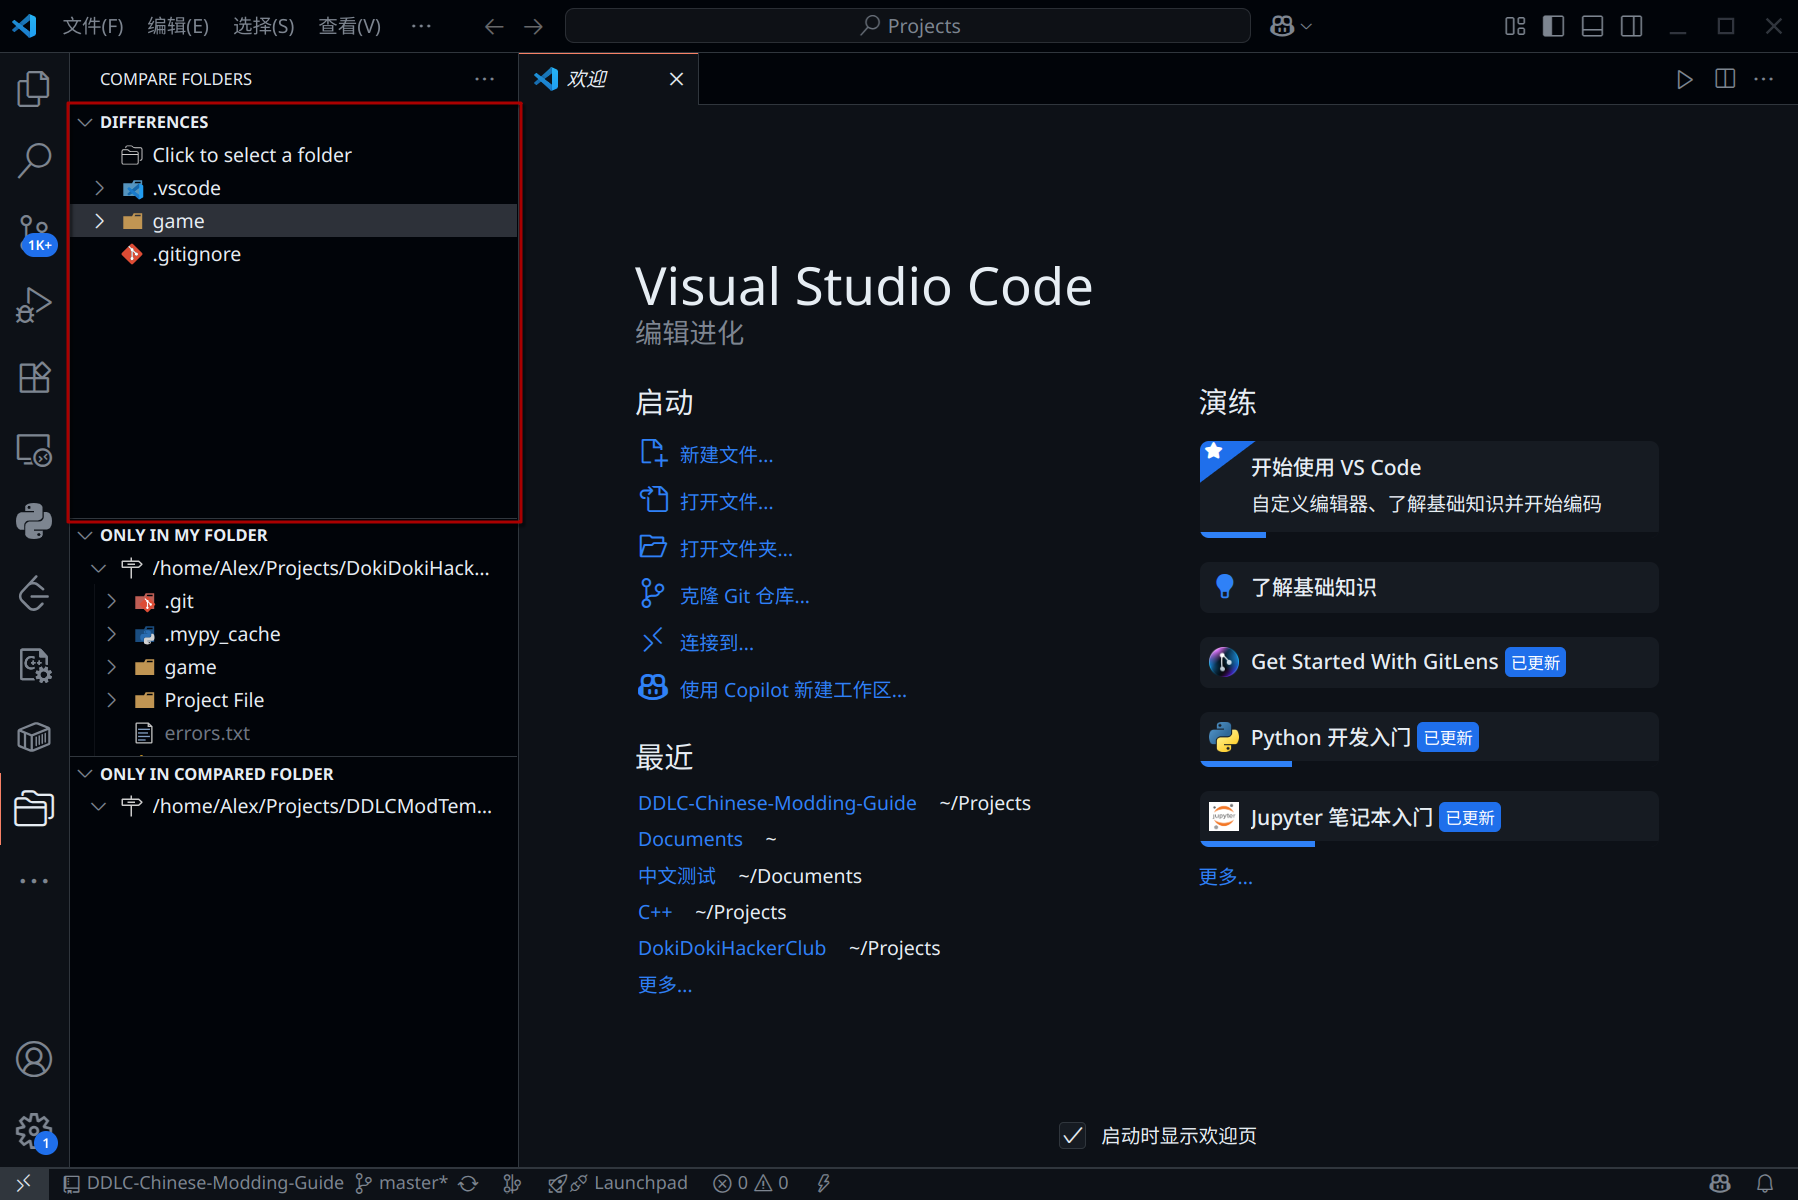
\includegraphics[scale=.2]{Pictures/7.1.2.1.png}
\end{figure}

在VS Code的文件选项卡中,选择新建窗口,在新的窗口中打开Future分支。回到原来的窗口,聚焦于“DIFFERENCES”栏目中,展开game文件夹,依次点击每个文件夹下的文件,查看文件的差异,并将修改过的代码同步修改到Future分支的对应文件下。

然后,聚焦于“ONLY IN COMPARED FOLDER”栏目中,这里是您添加的文件,将它们全部复制到Future项目中的对应位置。

到此,我们就完成了代码的迁移,接下来就是使用Ren'Py 8运行项目进行一轮完整的游戏,检测是否有代码运行结果在预期之外,并进行修复。

\subsection{解除兼容性警告}
初次运行项目,若您使用的Ren'Py版本高于8.0.3,您可能会遇到以下提示:

\begin{quote}
    \textbf{警告}:您目前用于开发 DDLC 模组的 Ren'Py SDK 未经过模组兼容性测试。

    目前最新的适用于 DDLC 模组的 Ren'Py 8 版本为\url{https://www.renpy.org/release/8.0.3}“Ren'Py 8.0.3”。
    
    在过高版本的 Ren'Py 上运行 DDLC 或其模组可能会引发问题,也可能导致游戏功能损坏。
\end{quote}

这个提示将会在初次运行时出现,原则上当您按照本指南的打包教程,将config.developer设置为False,那么这个提示将不会被展示。但以防万一,我们仍建议您从根源上取消该提示。

现在,关闭游戏,打开game/core/lockdown\_check.rpy文件,在label语句后添加一行,输入以下代码(注意缩进):
\begin{lstlisting}
    return
\end{lstlisting}

再次打开游戏,您会发现这段提示永久消失了。
